\section{Image segmentation}
Identify groups of pixels that belong together - goal: Delineate objects and background regions \& group similar-looking pixels for efficientcy of further processing

Examples of Groupin in vision
\begin{itemize}
	\item similar appearance
	\item symmetry
	\item common fate (direction etc)
	\item proximity
\end{itemize}

\subsection{Segmentation as clustering}
\subsubsection{Clustering}
Chicken and Egg problem  - either know the centers and allocate the points to it OR know the point membership and create center from them

Feature space - depending on that choice we can group pixels in different ways

\begin{itemize}
	\item pixel intensity
	\item pixel color
	\item pixel texture
	\item pixel intensity + position (proximity)
\end{itemize}

\subsubsection{k-Means}
Idea: randomly initialize the k cluster centers, and iterate between the two steps from clustering

Properties: will always converge to some solution (which can be a local maximum)

Pro:
\begin{itemize}
	\item simple, fast to compute
	\item converges (to local maximum)
\end{itemize}

Cons:
\begin{itemize}
	\item number of cluster has to be defined
	\item sensitive to initial centers
	\item sensitive to outliers
	\item detects spherical clusters only
	\item assuming means can be computed
\end{itemize}
\subsubsection{Mixture of Gaussians, EM}
Idea: instead of treating the data as a bunch of points, assume that they are all generated by sampling a continous function - this function is called a \textit{generative model}, defined by a vector of parameters $\theta$

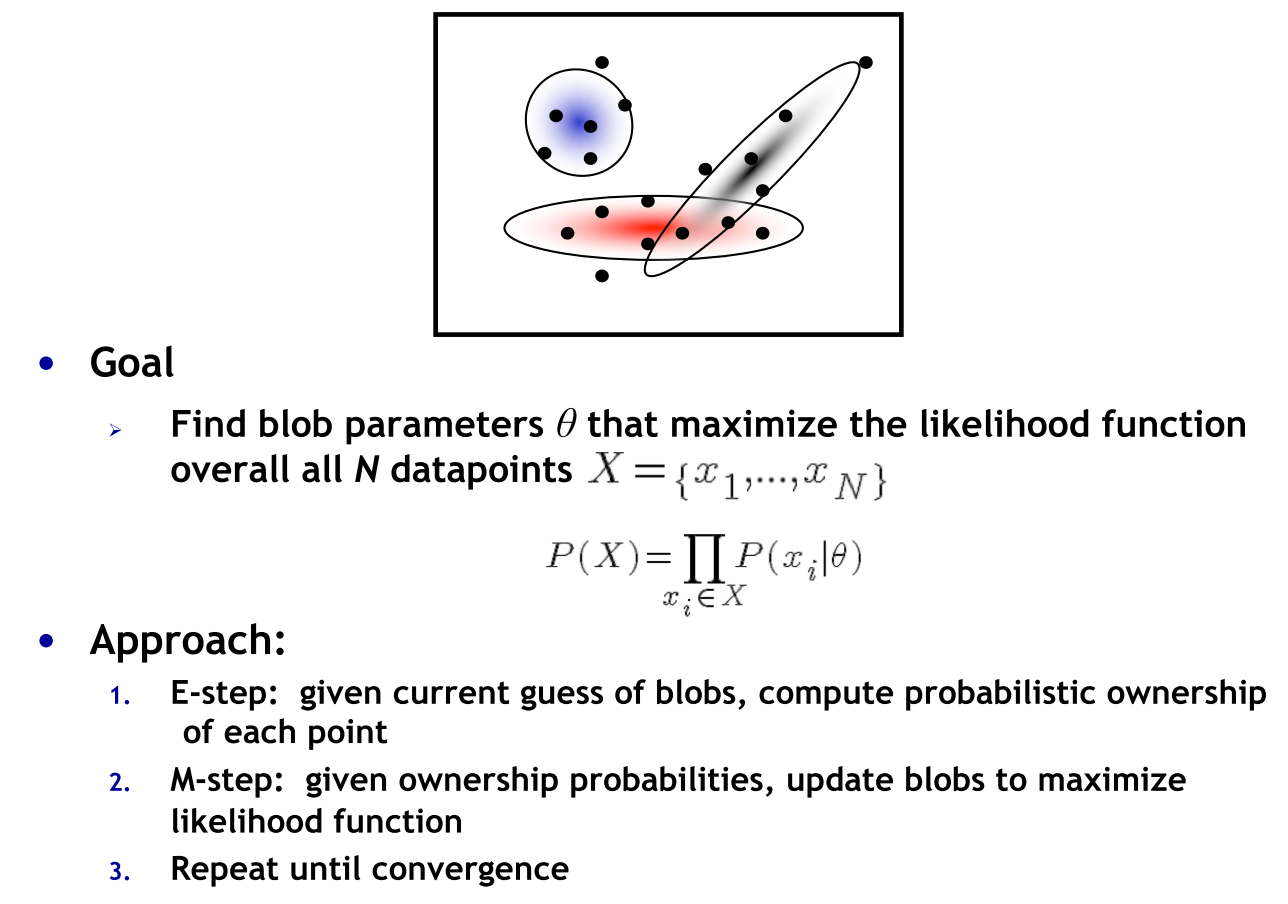
\includegraphics[width=\columnwidth]{pictures/EM}

E-Step: Compute probability that point $x$ is in blob b, given current guess of $\theta$

$$ P(b|x,\mu_b, V_b) = \frac{\alpha_b P(x|\mu_b, V_b)}{\sum_{i=1}^{K}\alpha_i P(x|\mu_i, V_i)} $$

M-Step: Compute overall probability that blob b is selected (N: data points)\\

Weight:
$$\alpha_b^{new} = \frac{1}{N} \sum_{i=1}^{N} P(b|x_i, \mu_b, V_b) $$
Mean of blob b:
$$ \mu_b^{new} = \frac{\sum_{i=1}^{N} x_i P(b|x_i, \mu_b, V_b)}{\sum_{i=1}^{N} P(b|x_i, \mu_b, V_b)}$$
Covariance of blob b:
$$ V_b^{new} = \frac{\sum_{i=1}^{N} (x_i-\mu_b^{new})(x_i-\mu_b^{new})^T P(b|x_i, \mu_b, V_b)}{\sum_{i=1}^{N} x_i P(b|x_i, \mu_b, V_b)} $$

EM Application is useful for all sorts of problems 
\begin{itemize}
	\item Any clustering problem
	\item Many model estimation problems
	\item Missing data problems
	\item Finding outliers
	\item Segmentation problems
	\begin{itemize}
		\item based on color
		\item based on motion
		\item Foreground/background separation 
\end{itemize}	
\end{itemize}
Pro:
\begin{itemize}
	\item Probabilistic interpretation
	\item Soft assignments between data points and clusters
	\item Generative model, can predict novel data points 
	\item Relatively compact storage ($O(Kd^2$)
\end{itemize}
Cons:
\begin{itemize}
	\item Initialization – often a good idea to start from output of k-means
	\item Local minima
	\item Need to know number of components K – Solutions: model selection (AIC, BIC), Dirichlet process mixture
	\item  Need to choose blob generative model (math form of a cluster?)
	\item Numerical problems are often a nuisance
\end{itemize}

\subsubsection{Mean-Shift Algorithm}
Choose features (color, gradients, texture, etc)
\begin{enumerate}
	\item Initialize random seed center and window size $W$
	\item Calculate center of gravity (the “mean”) of $W$: $ \sum_{x \in W} x H(x) $
	\item Shift the search window to the mean
	\item Repeat steps 2+3 until convergence for all centers
	\item merge windows that end up near the same peak/center
\end{enumerate}

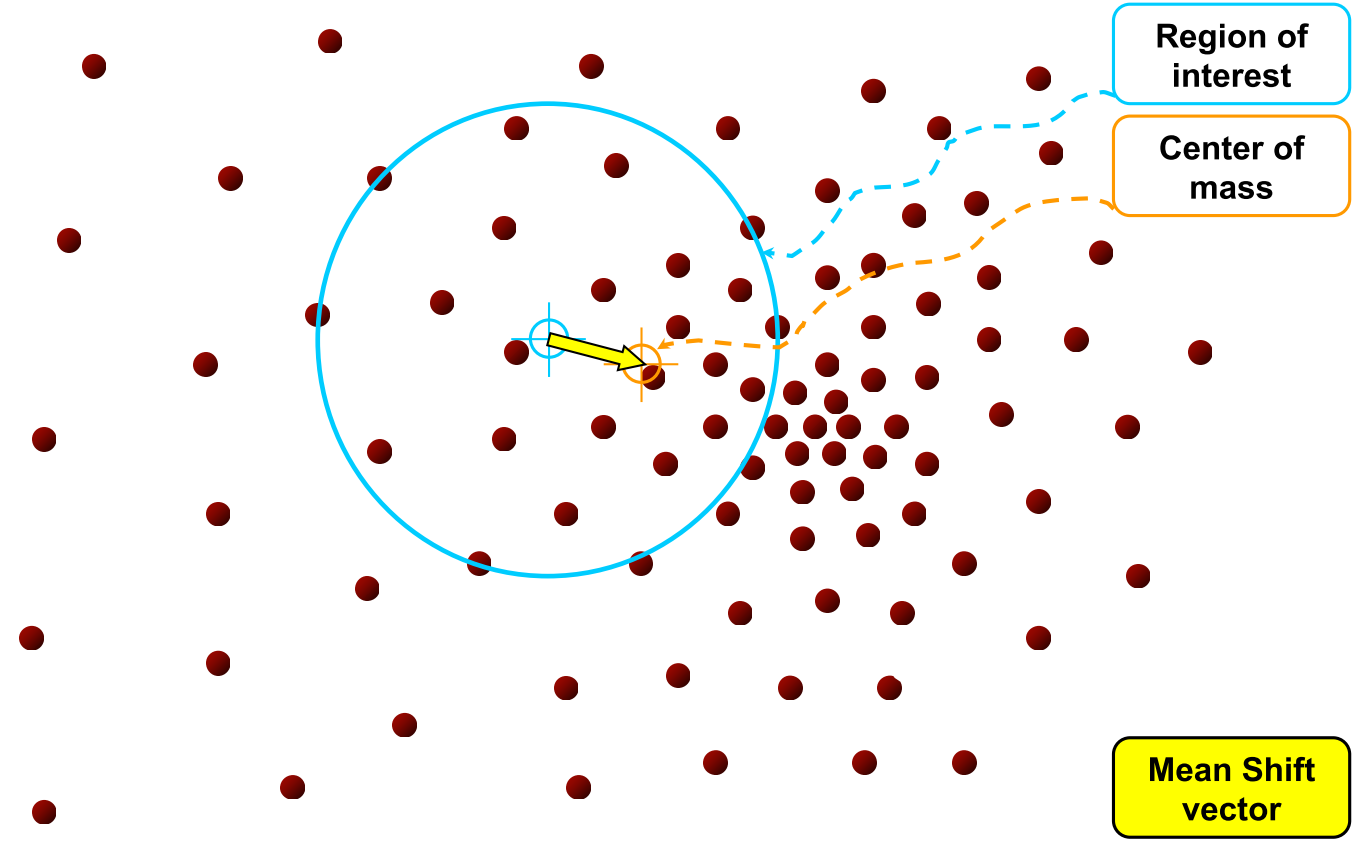
\includegraphics[width=\columnwidth]{pictures/meanshift}

Pro:
\begin{itemize}
	\item General, application-independent tool
	\item Model-free, does not assume any prior shape (spherical, elliptical, etc.) on data clusters
	\item Just a single parameter (window size h) – h has a physical meaning (unlike k-means) == scale of clustering
	\item Finds variable number of modes given the same h 
	\item Robust to outliers
\end{itemize}
Cons:
\begin{itemize}
	\item Output depends on window size h
	\item Window size (bandwidth) selection is not trivial
	\item Computationally rather expensive
	\item Does not scale well with dimension of feature space
\end{itemize}

\subsection{Hough transform}
see chapter before

\subsection{Interactive Segmentation with GraphCuts}
Markov Random Fields

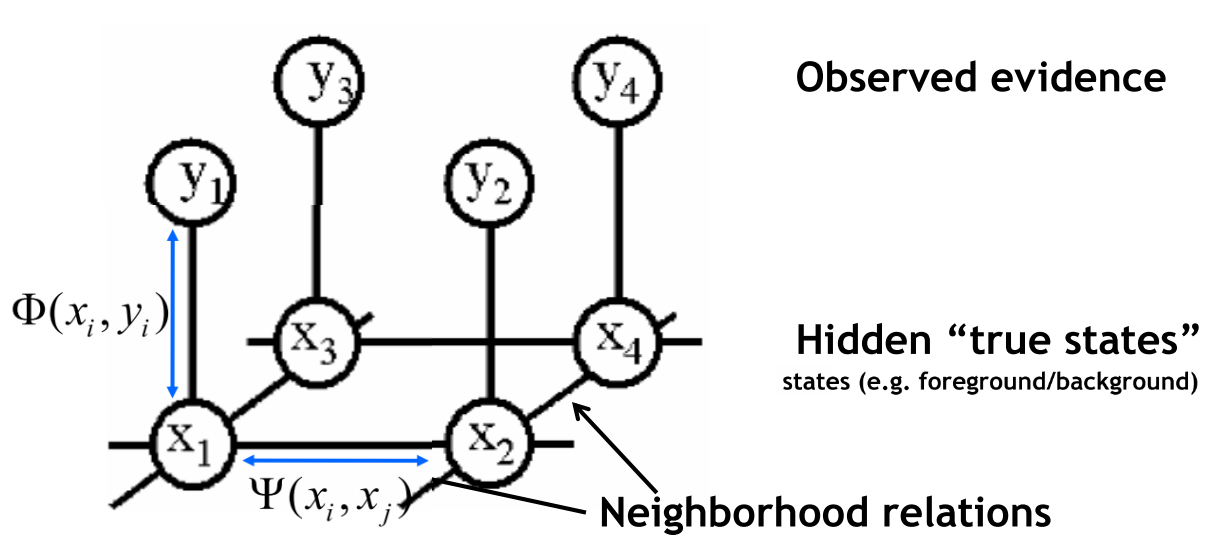
\includegraphics[width=\columnwidth]{pictures/markovfields}

Field Joint Probability

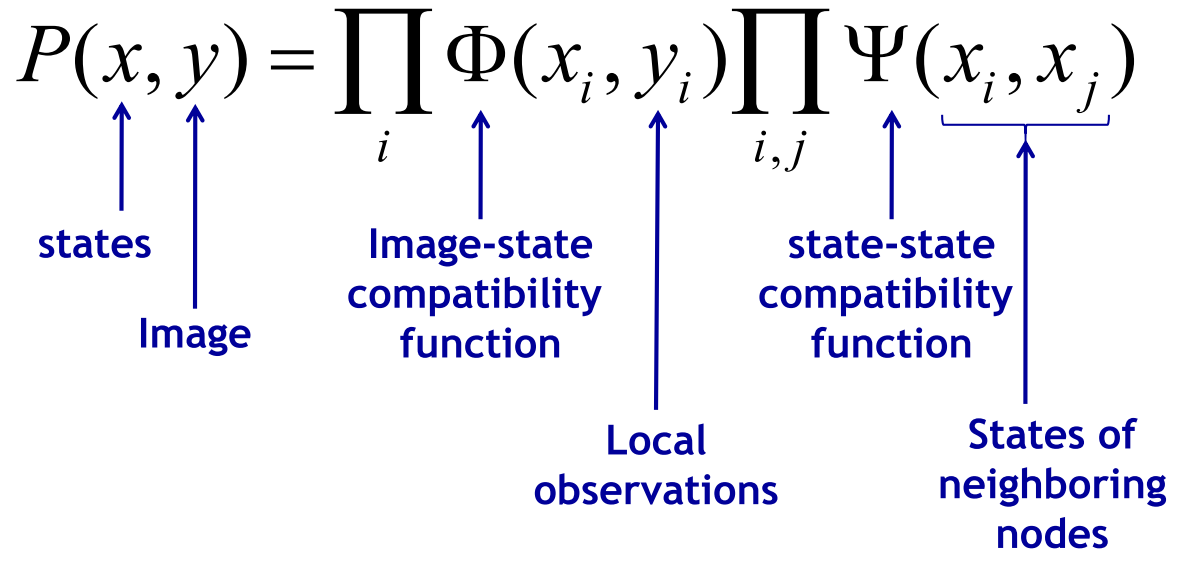
\includegraphics[width=0.7\columnwidth]{pictures/fieldjointprobability}

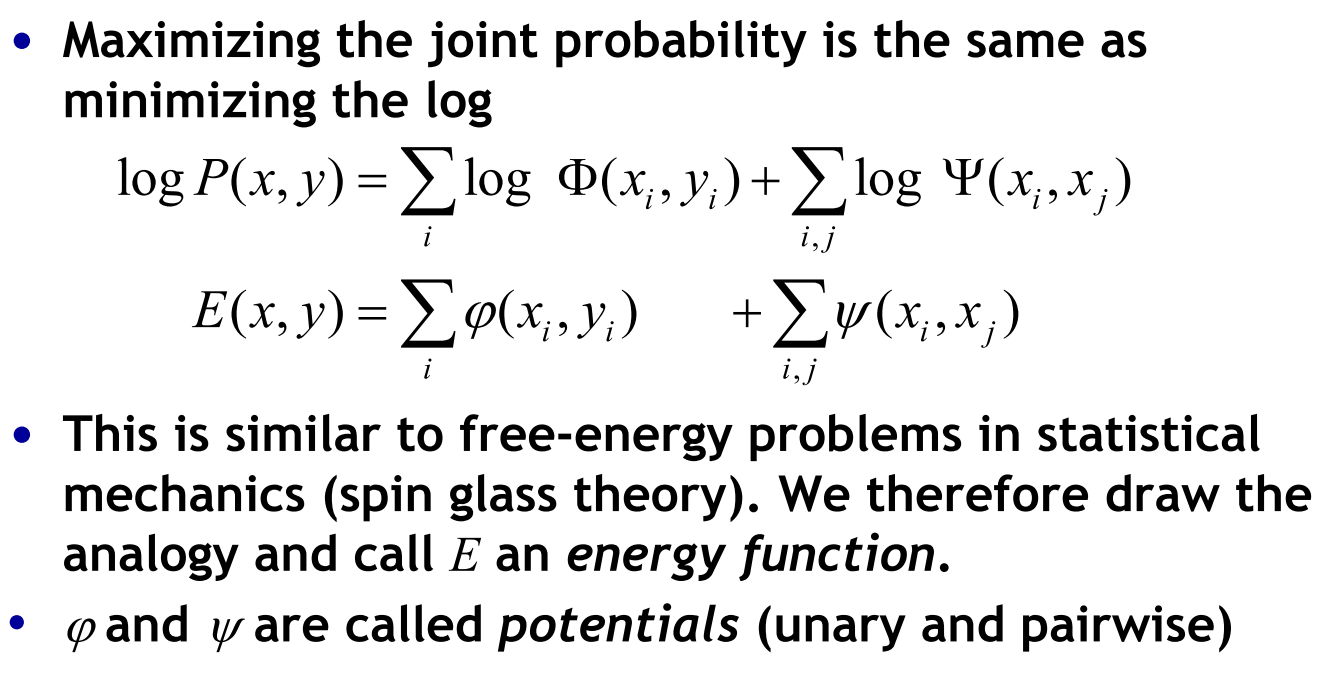
\includegraphics[width=\columnwidth]{pictures/energyfunction}
Unary potentials $\Phi$
\begin{itemize}
	\item Encode local information about the given pixel/patch
	\item How likely is a pixel/patch to be in a certain state (e.g. foreground/background)
\end{itemize}
Pairwise potentials $\Psi$
\begin{itemize}
	\item Ecode neighborhood information
	\item How different is a pixel/patch's label from that of its neighbor (e.g. here independent of image data, but later based on intensity/color/texture difference)
\end{itemize}

Goal: minimum cost cut

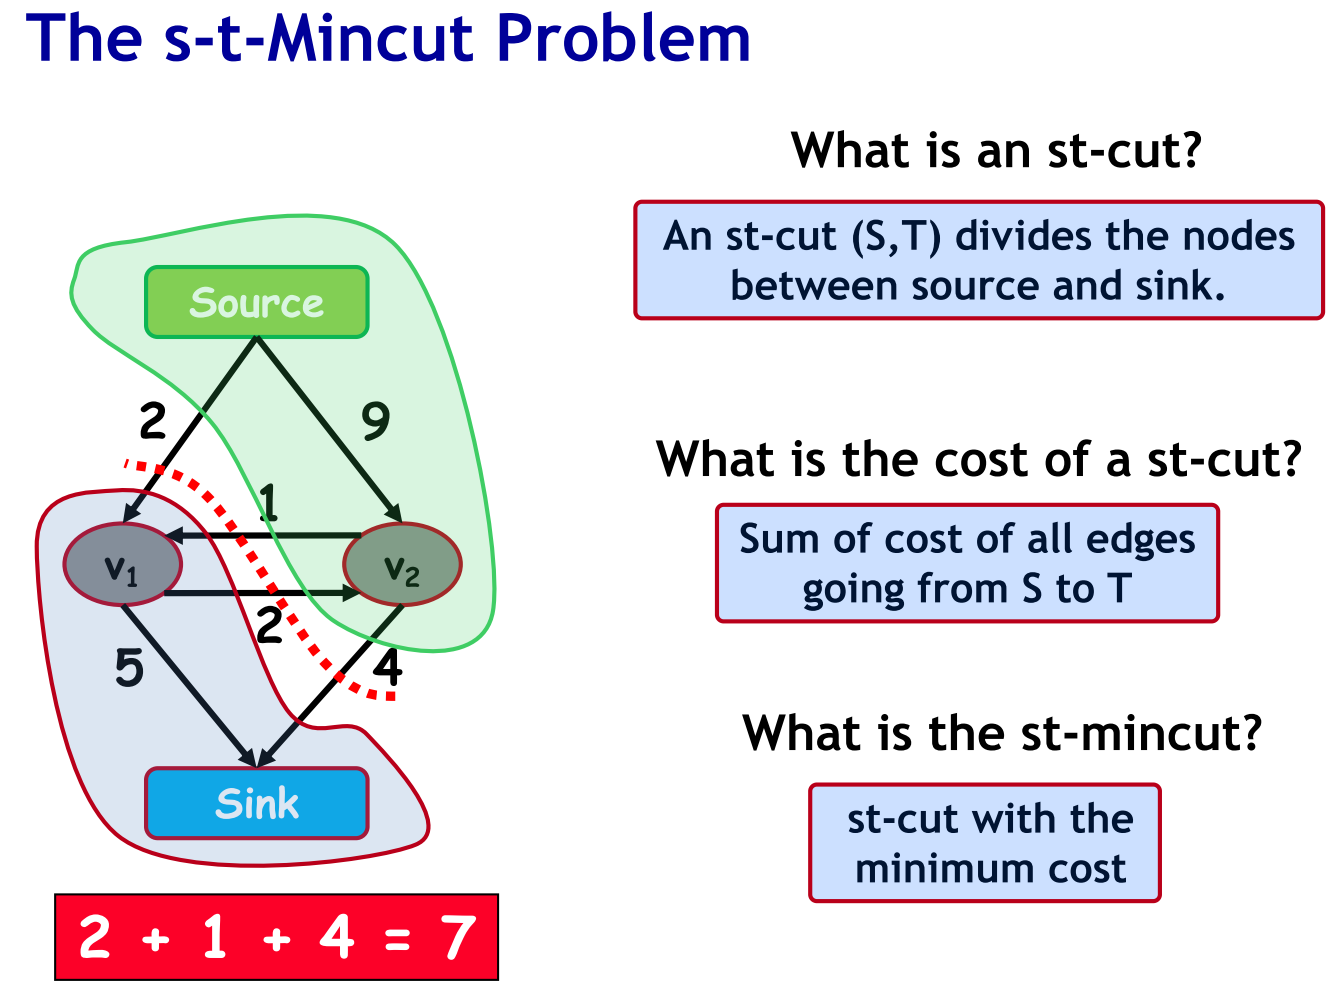
\includegraphics[width=\columnwidth]{pictures/s-t-min-cut}

Maxflow Algorithm
\begin{enumerate}
	\item Find path from source to sink with positive ! capacity
	\item push maximum possible flow through this path (subtract it from all segments)
	\item repeat until no path can be found
\end{enumerate}

Pro:
\begin{itemize}
	\item Powerful technique, based on probabilistic model (MRF).
	\item Applicable for a wide range of problems.
	\item Very efficient algorithms available for vision problems.
	\item Becoming a de-facto standard for many segmentation tasks.
\end{itemize}
Cons:
\begin{itemize}
	\item Graph cuts can solve a limited (but useful) class of models
	\item Submodular energy functions
	\item Can capture only part of the expressiveness of MRFs
	\item Only approximate algorithms available for multi-label case (except for special cases with particular topology and/or pairwise potentials)
\end{itemize}

\subsection{Learning-based approaches}
Extract the same features used during training \& Use the mapping learned before to label

\subsubsection{K-nearest neighbor}
For every point find the k nearest neighbors (labeled in the training set). The point is then defined through the lables of these neighbors (majority voting of these k neighbors)

Pro:
\begin{itemize}
	\item Very simple to implement
	\item Very simple to understand
	\item efficient implementations possible for approx. NNs
	\item distance definition is flexible
\end{itemize}
Cons:
\begin{itemize}
	\item highly depends on the definitions and k
	\item need to keep the entire data in memory for distance computations
	\item for high dimensional problems might need many training samples for accuracy
	\item other methods have better generalization ability
\end{itemize}

\subsubsection{Random forests}
Binary decision trees - Random Forests are slow to train, but fast to apply during testing.

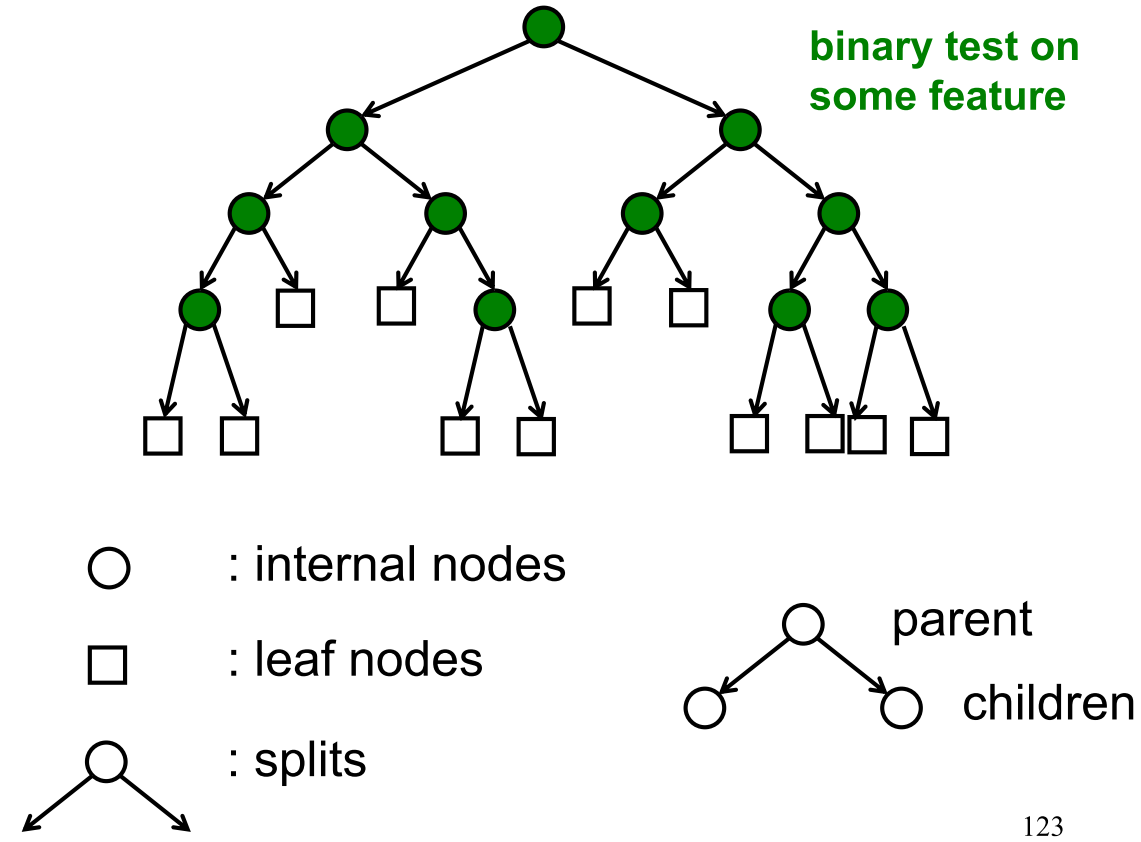
\includegraphics[width=\columnwidth]{pictures/tree}
TRaining: During training, samples are used for which the true class is known.
Having arrived at a node, one randomly generates a set of possible tests to carry out in order to split it up.
Among the possibilities one selects the test that maximally reduces the uncertainty. (biggest difference)\\
\\
Testing: Feed the current sample into every tree. See in which leaf node it ends -> (most probable) class. Combine the results, e.g. which class/label was found most often

Pro:
\begin{itemize}
	\item Easy to implement
	\item very efficient during testing
	\item can easily use diverse features
	\item can handle high dimensional spaces
\end{itemize}
Cons:
\begin{itemize}
	\item Lots of parametric choices
	\item needs large number of data
	\item training can take time
\end{itemize}